\documentclass{beamer}
\usetheme{Copenhagen}
\usepackage{graphicx}
\usepackage{tikz}
% \usepackage[ruled,vlined,english]{algorithm2e}
% \renewcommand{\thealgocf}{}
% \usepackage{hyperref}
\usepackage{unicode-math}
\usepackage{newunicodechar}
\newunicodechar{️}{}

\author[Jumeau numérique: Environnement]{\large Hanna CHETOUANE, Narmimane ZAOUACHE \\ \vspace{-0.8cm} \date{\today}}
\title[Microclimat urbain]{\textbf{Jumeau numérique dans l'environnement:} \\ Microclimat urbain}



\begin{document}

\begin{frame}
    \titlepage
    \vspace{-0.4cm}
    \begin{center}
        UFR of Mathematics and Informatics - University of Strasbourg 
        \\[0.2cm] 
        \textit{Comment les jumeaux numériques aident-ils à comprendre les effets des aménagements urbains sur le micro-climat ?}
    \end{center}
\end{frame} 


\begin{frame}{Plan}
    \tableofcontents    
\end{frame}


\begin{frame}{Contexte}
    \small
    \begin{itemize} % plus développer ?
        \item L'écologie et le climat sont devenus des enjeux majeurs, surtout dans les villes où se développent des îlots de chaleur
        \item Solutions: Végétalisation, choix de matériaux adaptés et aménagements urbains repensés
        \item Les collectiviités locales doivent ainsi prendre des décisions sur les stratégies d'aménagement à adopter et en évaluer l'impact environnemental et sanitaire
    \end{itemize}
    $\rightarrow$ Simuler et prédire ces effets de ces choix sur le microclimat urbain et la santé publique $\Rightarrow $ \textbf{Jumeau numérique}
\end{frame}


\begin{frame}{Qu'est-ce qu'un jumeau numérique ?}
    \small
    \begin{itemize}
        \item Réplique virtuelle et dynamique d'un système réel, qui, couplé à des outils de simulation, permet d'analyser et prédire son comportement dans différentes conditions
        \item S'appuie sur des données réelles (météorologiques et urbaines) issues de capteurs, d'observations ou de modèles physiques
    \end{itemize}
    \begin{center}
        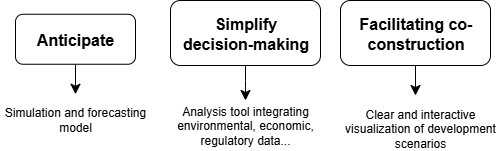
\includegraphics[width=0.7\textwidth]{images/objectifs_jm.png} \\
    \end{center}
    Défi actuel en France: projet JNFT porté par l'IGN, le Cerema et l'Inria, qui vise à créer un jumeau numérique multithématique couvrant le territoire français
\end{frame}


\begin{frame}{Fonctionnement d'un jumeau numérique} %Architecture et pipeline}
    \hspace*{-0.5cm}
    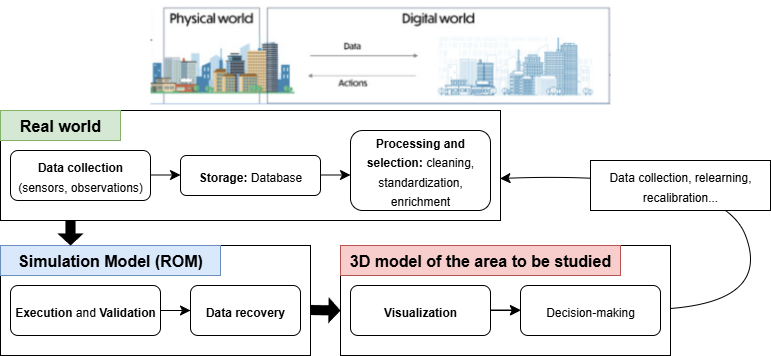
\includegraphics[width=1.1\textwidth]{images/pipeline.png} \\
\end{frame}


\begin{frame}{Méthodes}
    \small
    %Modélisation de phénomènes physiques
    % pour résoudre numériquement par FEM, VM, DM
    \begin{columns}[T]
        \begin{column}{0.45\textwidth}
            \textbf{Physique:} \\
            \begin{itemize}
                \item Données (météo, propriétés des matériaux, composition de l'air)
                \item Micro-climat
            \end{itemize}
        \end{column}
        \begin{column}{0.1\textwidth}
            \begin{center}
                \tikz[scale=1]{\draw[->, very thick] (0,0) -- (0.5,0);}
            \end{center}
        \end{column}
        \begin{column}{0.45\textwidth}
            \textbf{Numérique:}
            \begin{itemize}
                \item Paramètres
                \item Maquette 3D maillée
            \end{itemize}
            \vspace{0.3cm}
            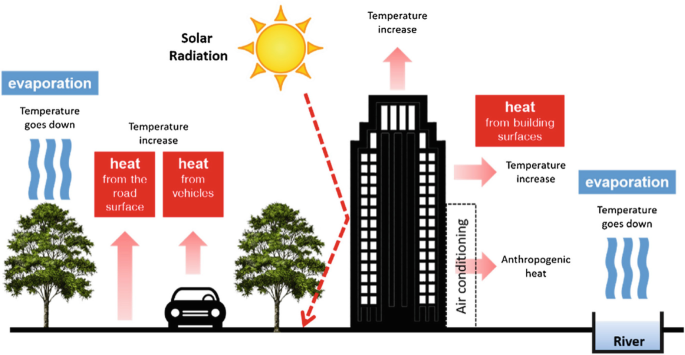
\includegraphics[width=0.7\textwidth]{images/micro-climat_scheme.png} \\
        \end{column}
    \end{columns}

    \vspace{-0.4cm}
    \textbf{Modèles physiques:}
    \begin{itemize}
        \item Phénomènes physiques continus: PDEs (Navier-Stockes, chaleur, transport, diffusion)
        \item Interaction entre batiments, vent, végétation: Fluid-Structure Interaction (NS + Elasticity)
        \item Ecoulement d'air et échanges thermiques: Computational Fluid Dynamics (NS + Heat; Transport; transfert radiatif) % effet du soleil sur les façades
    \end{itemize}
\end{frame}


\begin{frame}
    \small
    % résolution très lourde et longue à calculer, donc:
    \textbf{Utilisation ROM:} Réduction de l'ordre des modèles physiques pour accélérer les simulations  \\
    \vspace{0.2cm}
    - \textbf{Offline:} Préparation du modèle
    \begin{itemize}
        \item Réduction de la dimension en capturant l'essentiel du système: Proper Orthogonal Decomposition (POD), Reduced Basis Method (RBM)
        \item Hyper-réduction: Réduit temps de calcul des termes non-linéaires (DEIM: Discrete Empirical Interpolation Method, gappy POD: gappy Proper Orthogonal Decomposition) % en évaluant seulement certains points clés du modèle
    \end{itemize}
    \vspace{0.2cm}
    - \textbf{Online:} Simulation du modèle réduit pour tester différents scénarios rapidement
    \vspace{-0.4cm}
    \begin{flushright}
        \includegraphics[width=0.5\textwidth]{images/diff_scénarios.jpg}
    \end{flushright}
\end{frame}


\begin{frame}
    \small
    \textbf{Data-Driven Models:} basé sur les données, prédiction rapide % sur le micro-climat
    \begin{itemize}
        \item Régression: prédit des phénomènes (température, qualité de l'air, vent) à partir de variables (matériaux, végétation...) 
        \item Gaussian Process: prédit et donne l'incertitude pour des zones avec peu de données
    \end{itemize}
    \vspace{-0.3cm}
    \begin{columns}[T]
    \begin{column}{0.6\textwidth}
    \begin{itemize}
        \setlength\itemindent{0.3cm}
        \item Réseaux de Neuronnes: capture les relations complexes et non-linéaires entre les variables 
    \end{itemize}
    \end{column}

    \begin{column}{0.4\textwidth}
        \vspace{-0.3cm}
        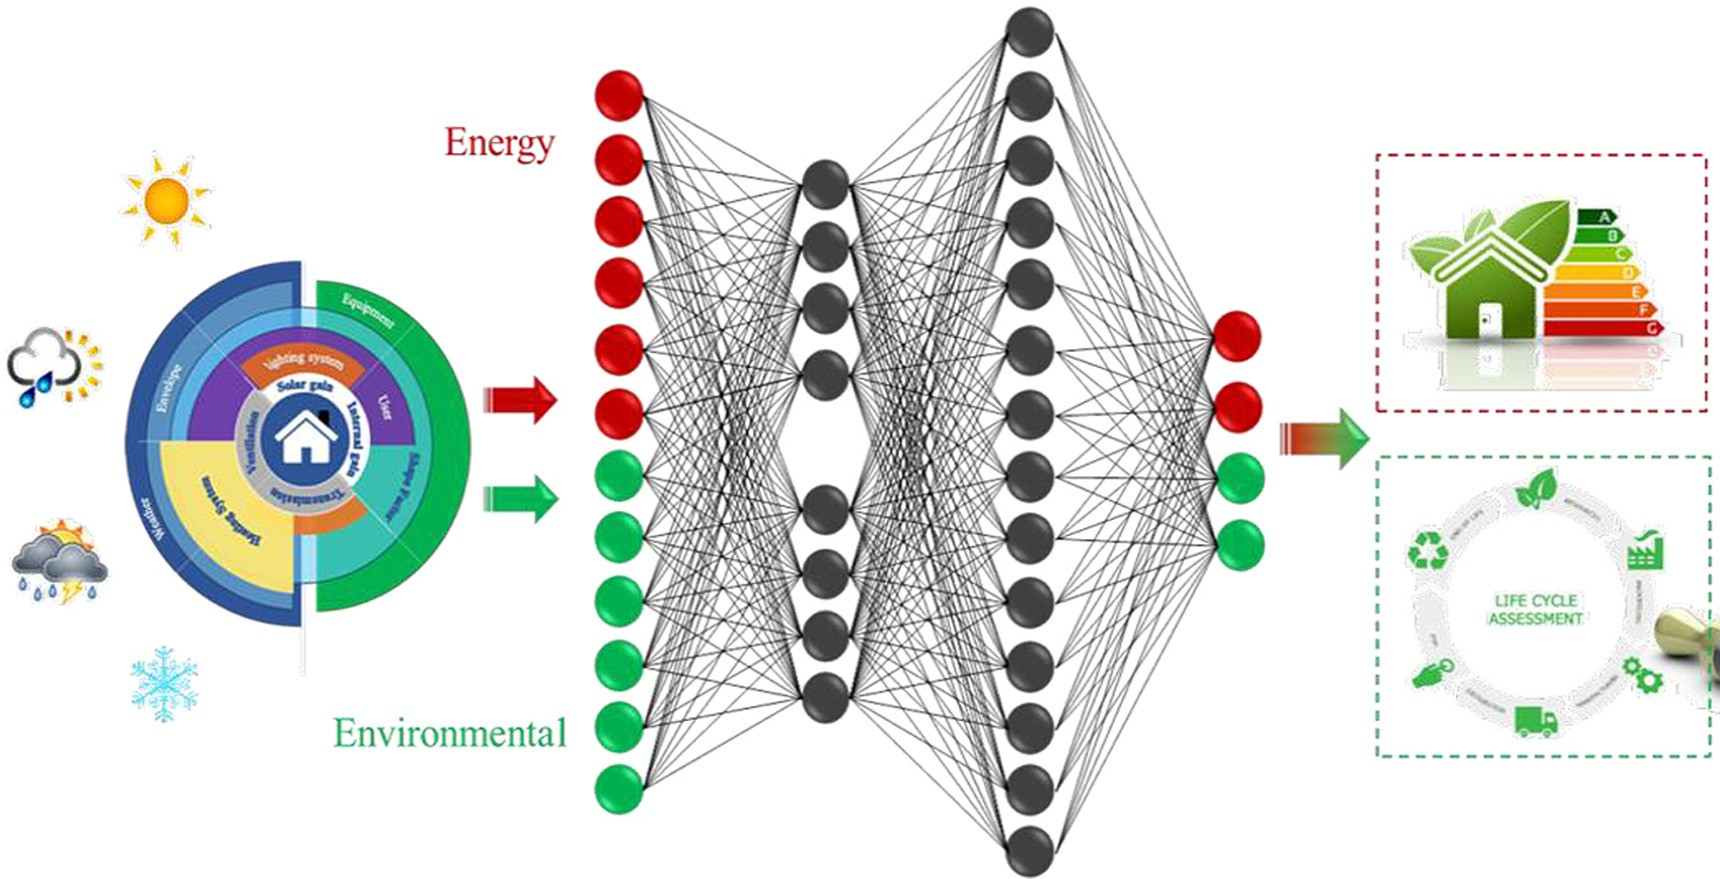
\includegraphics[width=1\textwidth]{images/NN-env.jpg}
    \end{column}
    \end{columns}
    \vspace{-0.3cm}
    \begin{itemize}
        \item Modèles d'ensembles: amélioration de \\ la précision et de la robustesse des prédictions, en combinant plusieurs modèles
    \end{itemize}
\end{frame}


\begin{frame}
    \small
    \textbf{Data assimilation:} Combinaison des modèles physiques et des données pour corriger les simulations, obtenir un maximum de précision et rendre ces simulations exploitables % pour la prise de décision
    \vspace{0.2cm}
    \begin{itemize}
        \item VAR: ajuste le modèle physique pour que les simulations collent aux observations (sur un ou plusieurs pas de temps)
        \item Filtre de Kalman: Mise à jour des prédictions en temps réel pour un suivi dynamique
        \item PBDW, GEIM: reconstruction du système avec peu de données, pour une vue d'ensemble
        \item Capteurs virtuels: estimation de variables où il n'y a pas de mesures, voir l'effet de nouveaux aménagements
    \end{itemize}
\end{frame}

\begin{frame}{Architecture and Pipeline}
\begin{columns}
    \begin{column}{0.55\textwidth}
        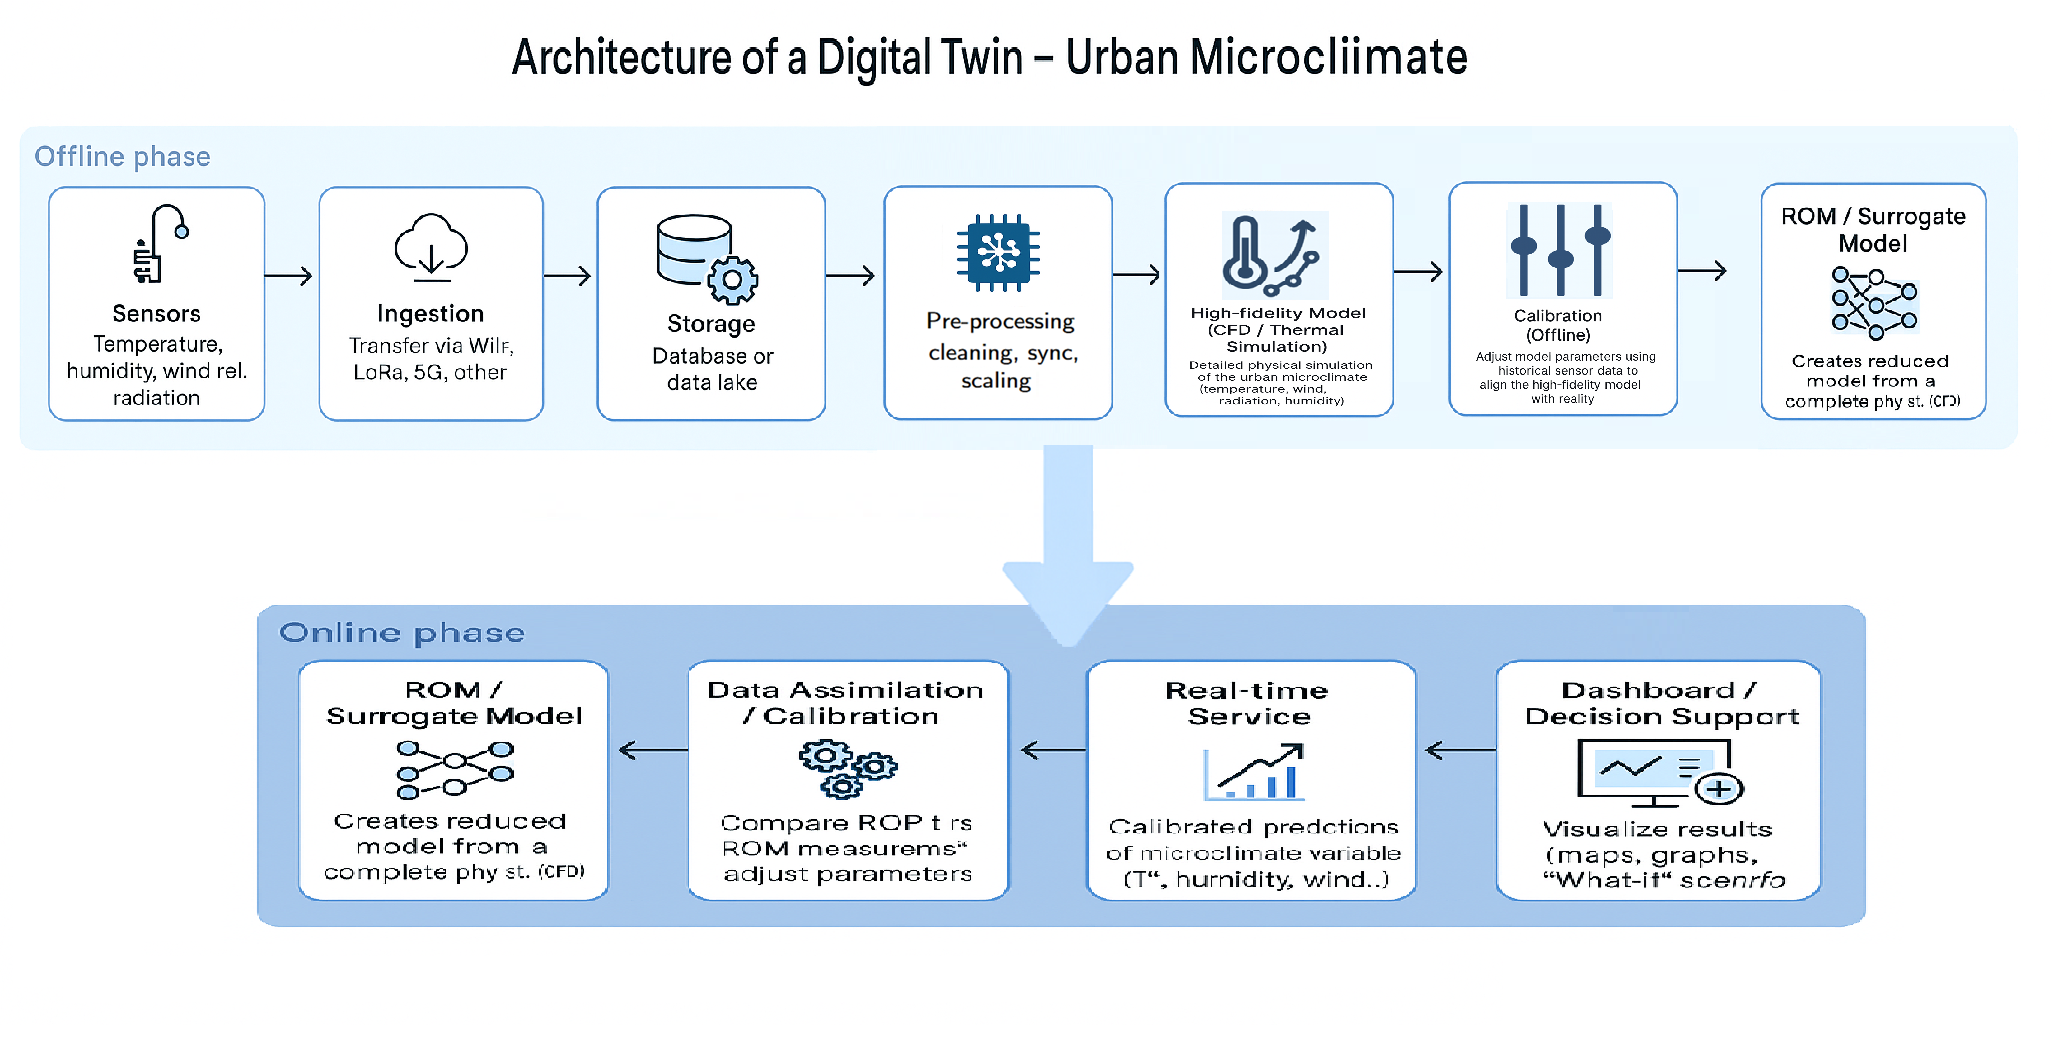
\includegraphics[width=\linewidth]{images/architecture_of_digital_twin.png}
    \end{column}
    \begin{column}{0.45\textwidth}
        \small
        The digital twin architecture is divided into two main phases:\\[4pt]
        \textbf{Offline:} model construction, calibration, and reduction.\\[3pt]
        \textbf{Online:} real-time assimilation and decision support.\\[4pt]
        This structure ensures continuous synchronization between the physical and virtual environments.
    \end{column}
\end{columns}
\end{frame}



\begin{frame}{Methods – Part 1: Physical and Reduced Models}
\small
\begin{block}{1. Physical and Numerical Modeling}
\begin{itemize}
    \item Based on fundamental equations (CFD, thermal transfer, radiation).
    \item Represents airflow, heat diffusion, and the effect of urban materials.
    \item Provides detailed simulations but is computationally expensive.
\end{itemize}
\end{block}

\begin{block}{2. Reduced Order Model (ROM / Surrogate Model)}
\begin{itemize}
    \item Built from the results of the high-fidelity physical model.
    \item Techniques: POD (Proper Orthogonal Decomposition), Reduced Basis Method (RBM), Hyper-reduction (DEIM).
    \item Enables calculations 100 to 1000 times faster while preserving accuracy.
\end{itemize}
\end{block}
\end{frame}


\begin{frame}{Methods – Part 2: Data-driven and Data Assimilation}
\small
\begin{block}{3. Data-driven Approaches (Machine Learning)}
\begin{itemize}
    \item Use sensor data to complement or correct physical models.
    \item Methods: regression models, neural networks (Neural-ODE), Gaussian Processes.
    \item Useful in areas with limited or missing physical data.
\end{itemize}
\end{block}

\begin{block}{4. Data Assimilation}
\begin{itemize}
    \item Continuously adjusts the model parameters using real-time measurements.
    \item Common methods: EnKF (Ensemble Kalman Filter), 4D-VAR, PBDW/GEIM.
    \item Keeps the digital twin consistent with the real environment in real time.
\end{itemize}
\end{block}
\end{frame}



\begin{frame}{Data \& Instrumentation — Data Budget (Urban Microclimate)}
\tiny
\setlength{\tabcolsep}{3pt}  
\textit{Goal: quantify sensor data rates and daily volumes to size network \& storage for real-time operation.}

\vspace{2mm}
\begin{tabular}{lcccccc}
\textbf{Sensor} & \textbf{\#} & \textbf{Freq (Hz)} & \textbf{sample} & \textbf{Throughput (kB/s)} & \textbf{Vol/day (GB)} & \textbf{Comments} \\
\hline
Air thermometer (T)   & 20 & 1.00  & 8        & 0.16  & 0.014 & Ambient temperature \\
Hygrometer (RH)       & 10 & 1.00  & 8        & 0.08  & 0.007 & Relative humidity \\
Anemometer (3-axis)   & 5  & 1.00  & 12       & 0.06  & 0.005 & Wind speed \& direction \\
Pyranometer (solar)   & 5  & 0.20  & 16       & 0.016 & 0.0014& Global irradiance \\
Thermal camera*       & 2  & 0.033 & 500{,}000& 33.0  & 2.85  & H.264, store temperature maps \\
\hline
\end{tabular}

\vspace{1mm}
\footnotesize
\textbf{Formulas:}
\begin{block}{Throughput (kB/s) \& Volume/day (GB)}
    $$Throughput (kB/s): \quad = \dfrac{\# \times \text{sample} \times \text{Freq}}{1000}$$
    $$ \noindent Volume/day (GB): \quad = \dfrac{\text{Throughput (kB/s)} \times 86\,400}{10^{6}}$$
\end{block}
\vspace{0.5mm}
\scriptsize
\textbf{Protocols/latency (summary):} LoRaWAN for low-rate sensors (2–5 s latency); Wi-Fi/4G for cameras ($<0.5$ s).  \\
\textbf{Privacy:} camera streams anonymized on edge; only thermal maps stored.
\end{frame}


\begin{frame}{V\&V \& UQ — Verification, Validation \& Uncertainty Quantification}
\centering
\tiny
\begin{block}{Goal}
    \textit{Goal: ensure accuracy, reliability, and safety of decisions in the urban microclimate digital twin.}
\end{block}
\vspace{0.4cm}
\begin{tabular}{|p{2.5cm}|p{3.5cm}|p{4.2cm}|}
\hline
\textbf{Step} & \textbf{Purpose} & \textbf{Methods / Indicators} \\
\hline
\textbf{1️⃣ Verification} &
Check model implementation and numerical stability. &
Compare the Reduced Order Model (ROM) with the full CFD model.  
Ensure no numerical or stability errors. \\
\hline
\textbf{2️⃣ Validation} &
Evaluate how well the model matches real-world data. &
Compare predictions with sensor measurements (T°, wind, humidity).  
Metrics: \textbf{MAE}, \textbf{RMSE}, \textbf{R\textsuperscript{2}}. \\
\hline
\textbf{3️⃣ Uncertainty Quantification (UQ)} &
Estimate the confidence level of model predictions. &
Methods: Monte Carlo, sensitivity analysis, Bayesian estimation.  
Example: $T = 32 \pm 1.5^\circ$C. \\
\hline
\textbf{4️⃣ Veto / Alert Mechanism} &
Prevent wrong or unsafe decisions when uncertainty is too high. &
If variance or RMSE $>$ threshold → trigger alert or model recalibration. \\
\hline
\end{tabular}

\vspace{0.3cm}
\textit{Outcome: a validated, uncertainty-aware model ensuring trustworthy real-time decisions.}
\end{frame}


\begin{frame}{Transfer \& Deployment — CI/CD, Edge vs Cloud, Observability, Risks}
\centering
\tiny
\begin{block}{Goal}
    \textit{ensure a smooth transition from R\&D to real-time operation of the urban microclimate digital twin.}
\end{block}
\vspace{0.4cm}
\begin{tabular}{|p{2.5cm}|p{3.5cm}|p{4.2cm}|}
\hline
\textbf{Aspect} & \textbf{Description} & \textbf{Tools / Key Points} \\
\hline
\textbf{CI/CD (Continuous Integration \& Deployment)} &
Automate the update cycle for models and data. &
GitHub Actions, Docker, unit tests for ROM/data, dashboard updates. \\
\hline
\textbf{Containers \& Orchestration} &
Ensure portability and scalability of digital twin services. &
Docker / Kubernetes: deployment of ROM model, APIs, dashboards. \\
\hline
\textbf{Edge vs Cloud Computing} &
Balance local computing (edge) and centralized storage (cloud). &
Edge: low latency (cameras, sensors).  
Cloud: heavy computations (assimilation, ROM training). \\
\hline
\textbf{Observability \& Monitoring} &
Track performance, errors, and model drifts. &
Logs, metrics, and alerts through Grafana / Prometheus. \\
\hline
\textbf{Costs \& Risks (CAPEX/OPEX)} &
Optimize hardware resources and minimize downtime. &
CAPEX: servers / sensors.  
OPEX: maintenance, energy, network.  
Risk: failure, model drift. \\
\hline
\end{tabular}

\vspace{0.3cm}
\textit{Outcome: a reliable, automated, and maintainable digital twin for long-term operation.}
\end{frame}


\begin{frame}{Perspectives \& Limitations — Toward a Sustainable Digital Twin}

\vspace{3mm}
\begin{itemize}
    \item 🔹 \textbf{Scalability:} adapt the model to larger urban areas (optimized ROM, cloud computation).  
    \item 🔹 \textbf{Robustness:} handle sensor failures or noisy data (redundancy, adaptive models).  
    \item 🔹 \textbf{Bias:} avoid overfitting to one district (multi-scenario validation).  
    \item 🔹 \textbf{Privacy:} ensure GDPR compliance and anonymization of visual data.  
    \item 🔹 \textbf{Ethics:} promote transparency, explainable AI, and citizen involvement.  
\end{itemize}

\end{frame}


% --- Slide: Acknowledgment / Questions ---
\begin{frame}{Thank You / Questions}
\centering
\Huge \textbf{Thank you for your attention!} \\
\vspace{1cm}
\Large Any questions? \\
\vspace{0.5cm}
\textit{University of Strasbourg – 2025}
\end{frame}




%\begin{frame}{Bibliographie}
    % https://www.ign.fr/institut/un-jumeau-numerique-de-la-france-pour-piloter-la-transition-ecologique
    % https://cnig.gouv.fr/IMG/pdf/2025.01_20_jnft_presentation_cnig_pole_territoires.pdf
    % Fondateurs de la démarche: IGN, Cerema, Inria
    % slide 10 -> 30% pour les aménagements durables
    % https://www.sciencedirect.com/science/article/pii/S2212095525002469
%\end{frame}



% --- Slide: Références ---
\begin{frame}[allowframebreaks]{Références}
  \nocite{*}
  \bibliographystyle{plain}
  \bibliography{bibliography}
\end{frame}


\end{document}